\scanpage{38}
\mspage{\handwritten{6}}
% archive sheet number: 37

\margin{\handwritten{\figure{
\begin{tikzpicture}[scale=.75]
\node[rotate=25,inner sep=1pt] at (0,0) {interchange};
\draw[rotate=25] (0,0) ellipse (1.05 and .27);
\end{tikzpicture}}}}
Given that the $\handwritten{\unsure{\mathscr{A}|\mathcal{A}}}_i$ are \deleted{\unsure{not}} noetherian rings, this makes it possible in many\inserted{\handwritten{cases}} to pass
% The typed words retain their positions; the circles and transposition arrow are handwritten.
\figure{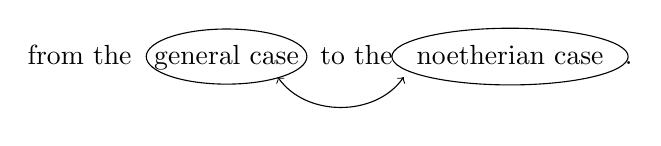
\begin{tikzpicture}
\node[anchor=base east,inner sep=0pt] at (-1.2,0) {from the};
\node[anchor=base,inner sep=0pt] at (0,0) {general case};
\node[anchor=base,inner sep=0pt] at (1.65,0) {to the};
\node[anchor=base,inner sep=0pt] at (3.6,0) {noetherian case};
\node[anchor=base west,inner sep=0pt] at (5.05,0) {.};
\handwritten{\draw (0,.10) ellipse (1.02 and .35);
\draw (3.6,.10) ellipse (1.50 and .36);
\draw[<->] (.65,-.16) to[out=-55,in=-125] (2.25,-.16);}
\end{tikzpicture}}

We shall now give two results concerning the particular case considered in a).

\uline{Proposition 10.11.}- \uline{Let $S$ be an integral prescheme with generic point $\handwritten{\eta}$, $G$ an $S$-group of finite presentation, $X$ an $S$-prescheme of finite presentation, $u$ and $v$ two $S$-morphisms from $X$ to $G$, $i:H\handwritten{\longrightarrow}G$ and $j:K\handwritten{\longrightarrow}G$ two monomorphisms of finite presentation. Then :}

\uline{(i) there exists a nonempty open subset $S'$ of $S$ such that if we denote by $G'$ (resp $H'$, resp. $X'$, resp $u'$, resp $v'$) the restriction of $G$(resp. $H$,resp. $X$, resp. $u$,resp. $v$) over the open subset $S'$ of $S$, the functor\deleted{\unsure{s}} $\underline{\operatorname{Transp}}(u',v')$ (resp. $\underline{\operatorname{Centr}}(u')$, $\underline{\operatorname{Centr}}_{G'}H')$ is representable by a closed $S'$-subprescheme of finite presentation $T'_1$ (resp. $C'_1$, resp. $C'_2$) of $G'$.}

\uline{(ii) suppose that $K_{\handwritten{\eta}}$ is closed in $G_{\handwritten{\eta}}$ (which is the case if $K$ is a subgroup $\deleted{p}S$-prescheme of $G$ (1.4.2)); then there exists a nonempty open subset $S'$ of $S$ such that if we denote by $G'$ (resp. $H'$, resp. $K'$) the restriction of $G$ (resp. $H$, resp. $K$)over the open subset $S'$ of $S$, the functor $\underline{\operatorname{Transp}}_{G'}(H',K')$ (resp. $\underline{\operatorname{Norm}}_{G'}K')$ is representable by a closed $S'$-subprescheme of finite presentation $T'_2$ (resp. $N'$) of $G'$.}

\uline{(iii)suppose that $H_{\handwritten{\eta}}$ and $K_{\handwritten{\eta}}$ are closed in $G_{\handwritten{\eta}}$ (which is the case if $H$ and $K$ are subgroup preschemes of $G$ (1.4.2)); then there exists} \inserted{\handwritten{an open}} \uline{nonempty subset $S'$ of $S$ such that if we denote by $G'$ (resp $H'$, resp. $K'$) the restriction of $G$ (resp. $H$, resp. $K$) over the open subset $S'$ of $S$, the functor $\underline{\operatorname{Transpstr}}_{G'}(H',K')$ is representable by a closed $S'$-subprescheme of finite presentation of $G'$.}

Since $G_{\handwritten{\eta}}$, $X_{\handwritten{\eta}}$, $H_{\handwritten{\eta}}$, $K_{\handwritten{\eta}}$ are flat over the field $\handwritten{\kappa}(\handwritten{\eta})$, and since
